\section{Property Graph Matching Framework}\label{sec:framework}
\begin{figure}[ht]
  \centering
  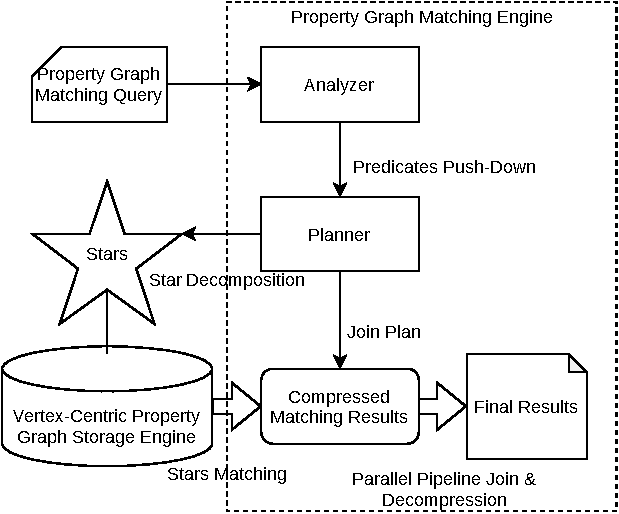
\includegraphics[width=0.48\textwidth]{img/architecture.pdf}
  \caption{The workflow of our property graph matching framework.}\label{img:architecture}
\end{figure}
Figure~\ref{img:architecture} shows the workflow of our property graph matching framework and Figure~\ref{img:pattern_graph} shows a diamond property graph which is a famous pattern in recommendation systems~\cite{DBLP:journals/pvldb/GuptaSGGZLL14}.
Unlike the simple graph model that has been well studied,
the property graph model is much more complex:
A graph is directed where both vertices and edges are labeled, and multiple edges may exist between two vertices.
Because of the complexity of the real-world property graphs,
a simple in/out-edges storage method is not suitable and would incur many unnecessary random disk accesses.
To address these problems, we develop a vertex-centric property graph storage model in Section~\ref{sec:storage}.
Based on the storage model, in Section~\ref{sec:match},
we propose a property graph matching engine that is able to solve real-world problems by leveraging the economical disk.

A graph matching query consists two parts: the pattern graph description part (the MATCH clause) and the constraint specification part (the WHERE clause).
In order to demonstrate the workflow clearly,
consider the Cypher query in Figure~\ref{img:cypher_query} which corresponds to the pattern graph in Figure~\ref{img:pattern_graph}.
Since tree-based graph matching algorithms have to scan the data graph randomly,
which is not suitable for out-of-core systems,
a join-based graph matching algorithm is preferable and the key is to determine the basic join unit.
The basic unit should be simple enough to avoid complex indices and complex enough to reduce intermediate matching results, therefore, we use stars to make the balance.
With the help of our property graph storage engine, we could scan the huge data sequentially only once (Section~\ref{sec:match_star}).
As is shown in Figure~\ref{img:compress_example}, the matching results of stars could still explode because of the expensive Cartesian product.
To address this challenge, we develop a compression method to reduce the I/O cost to materialize the stars' matching results in Section~\ref{sec:match_compress}.
And Section~\ref{sec:match_join} discusses the pipeline join method to join on the compressed matching results.
Moreover, previous works usually ignore the constraint specification part and leave them until the final results are obtained to filter out unnecessary ones,
however, we found that the WHERE clause usually contains many useful pruning information and we propose optimizations to push them down to the graph matching phase in Section~\ref{sec:match_optimize}.
\begin{figure}[ht]
  \begin{minted}[fontsize=\scriptsize]{cypher}
    MATCH (u1:Person)-[:FOLLOWS]->(u2:Person)-[:FOLLOWS]->(u1),
          (u1)-[:FOLLOWS]->(u3:Person)-[:FOLLOWS]->(u1),
          (u1)-[:PUBLISHES]->(u4:Media), (u1)-[:LIKES]->(u4),
          (u2)-[:LIKES]->(u4)<-[:LIKES]-(u3)
    WHERE id(u1) < id(u2) AND id(u1) < id(u3) AND
          NOT (id(u2) >= id(u3) OR id(u4) >= 2020)
  \end{minted}
  \caption{Graph matching query of the pattern graph in Figure~\ref{img:pattern_graph}.}\label{img:cypher_query}
\end{figure}
\begin{figure}[ht]
  \centering
  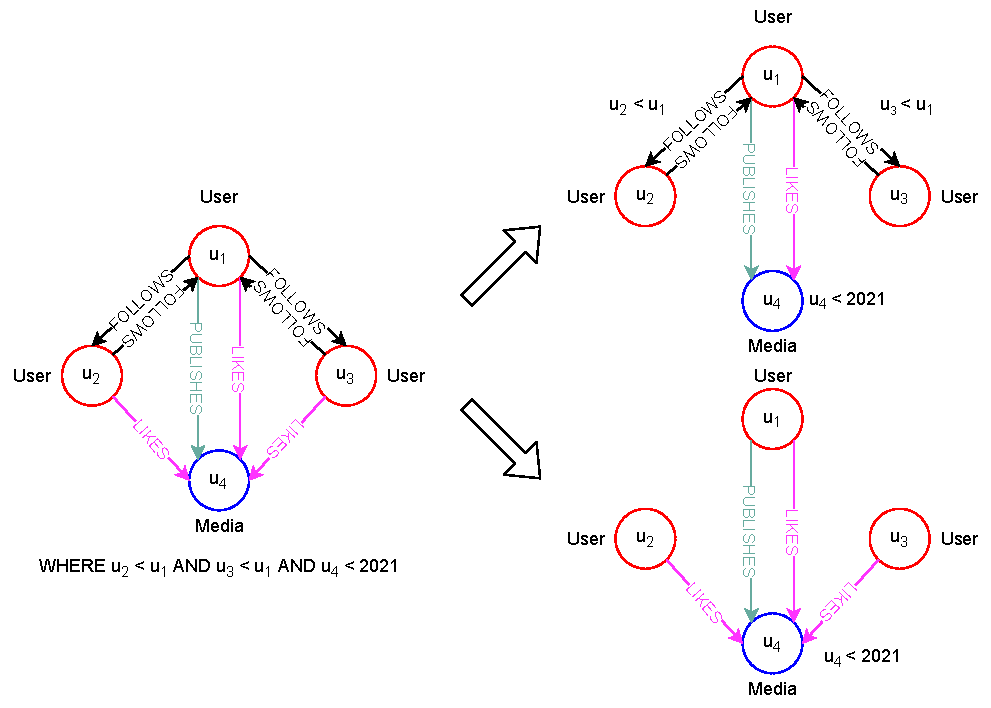
\includegraphics[width=0.48\textwidth]{img/pattern_graph.pdf}
  \caption{A pattern for recommendation system of social network and the decomposition of stars.}\label{img:pattern_graph}
\end{figure}
